\section{Conclusion}
\label{sec:conclusion}

The objective of the laboratory is to transform an input AC voltage of 230V in Hz to an output of 12V, while minimizing the ripple, deviation of said 12V and cost. As shown in Table~\ref{tab:CONCLUSAO}, the simulation results obtained have non trivial diferences to presented results already expected by the theoretical analysis achieved by Octave and Ngspice simulator. In fact, the relative error between the distances is of the magnitude of $10^2$ and the relative error between the ripples is of the magnitude of $10^3$.

The differences in theoretical analysis is the result of the diode model being different from the one used in the simulation model. Theoretical analysis uses a more simplified diode model than the one used in the simulation, although, we can say that in general a theoretical analysis is acceptable, as it is less complex and still presents good results.

The greater the complexity of the models used, the results can be more and more divergent between the theoretical analysis and a simulation, specialy while considering that the envelope is fully independent of the voltage regulator ande vice versa. If it is not the case, then the results would different regardless of other aproximations used in the theoretical analysis.

The tables with the results are the following:

\begin{table}[h]
\centering
\begin{minipage}[t]{0.33\linewidth}
 	 \begin{tabular}[t]{|l|r|}
 	   \hline    
 	   {\bf Name} & {\bf Value [A or V]} \\ \hline
 	   \input{../mat/MAT_tab}
 	 \end{tabular}
 	 \label{tab:TEO_CONCLUSAO}
\end{minipage}
\begin{minipage}[t]{0.33\linewidth}
  		\begin{tabular}[t]{|l|r|}
    	\hline    
   		{\bf Name} & {\bf Value [A or V]} \\ \hline
    	n & 0.56882248\\ \hline
cost & 302.2\\ \hline
mean(v(3))-12 & 5.094465e-07\\ \hline
vecmax(v(3))-vecmin(v(3)) & 8.328428e-04\\ \hline
1 / (abs(mean(v(3))-12) + vecmax(v(3))-vecmin(v(3)) + 1u) / (150+150+(18 + 4)*.1) & 3.966031e+00\\ \hline

  		\end{tabular}
  	\label{tab:SIM_CONCLUSAO}
\end{minipage}
  	\caption{Results in Octave and NGSpice, respectivily. Merit is in {\it per voltage per cost} and expressed in Volt$^{-1}$UC$^{-1}$; other variables are of type {\it voltage} and expressed in Volt. (As shown in Tables \ref{tab:TEO_RES} and \ref{tab:SIM_RES})}
  	\label{tab:CONCLUSAO}
\end{table}

The Merit result was 3.966 $V^{-1}uc^{-1}$ by Ngspice. It was agreed by the members of the group that the main goal of task was completed.
\newpage
The obtained plot with NGSpice and Octave are the following:

\begin{figure}[h] \centering
	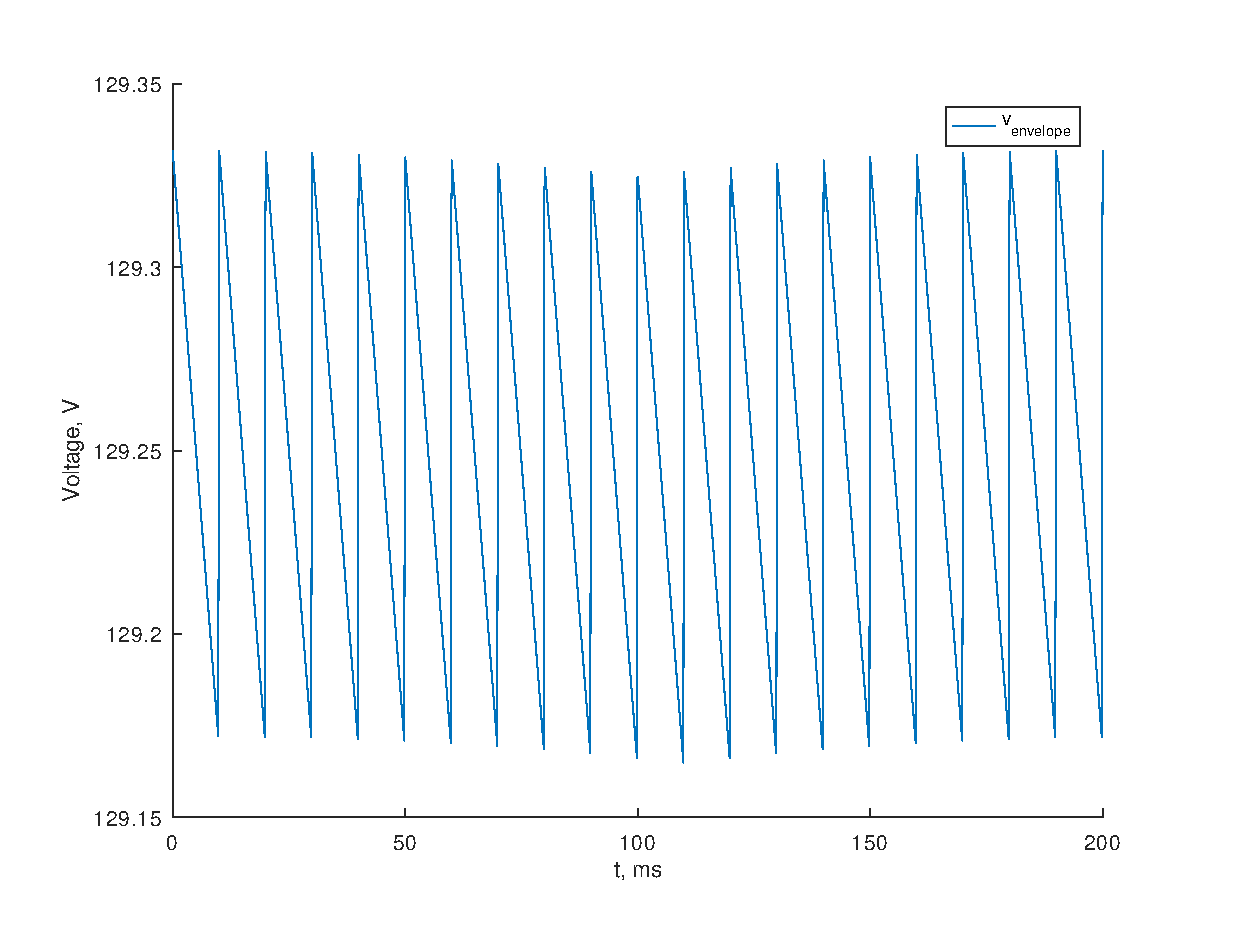
\includegraphics[height=8cm]{PASSO41.eps}
	\caption{Envelope detector $V_{envelope}$.}
\end{figure}
  	
\begin{figure}[h] \centering
	\vspace{-2cm}
	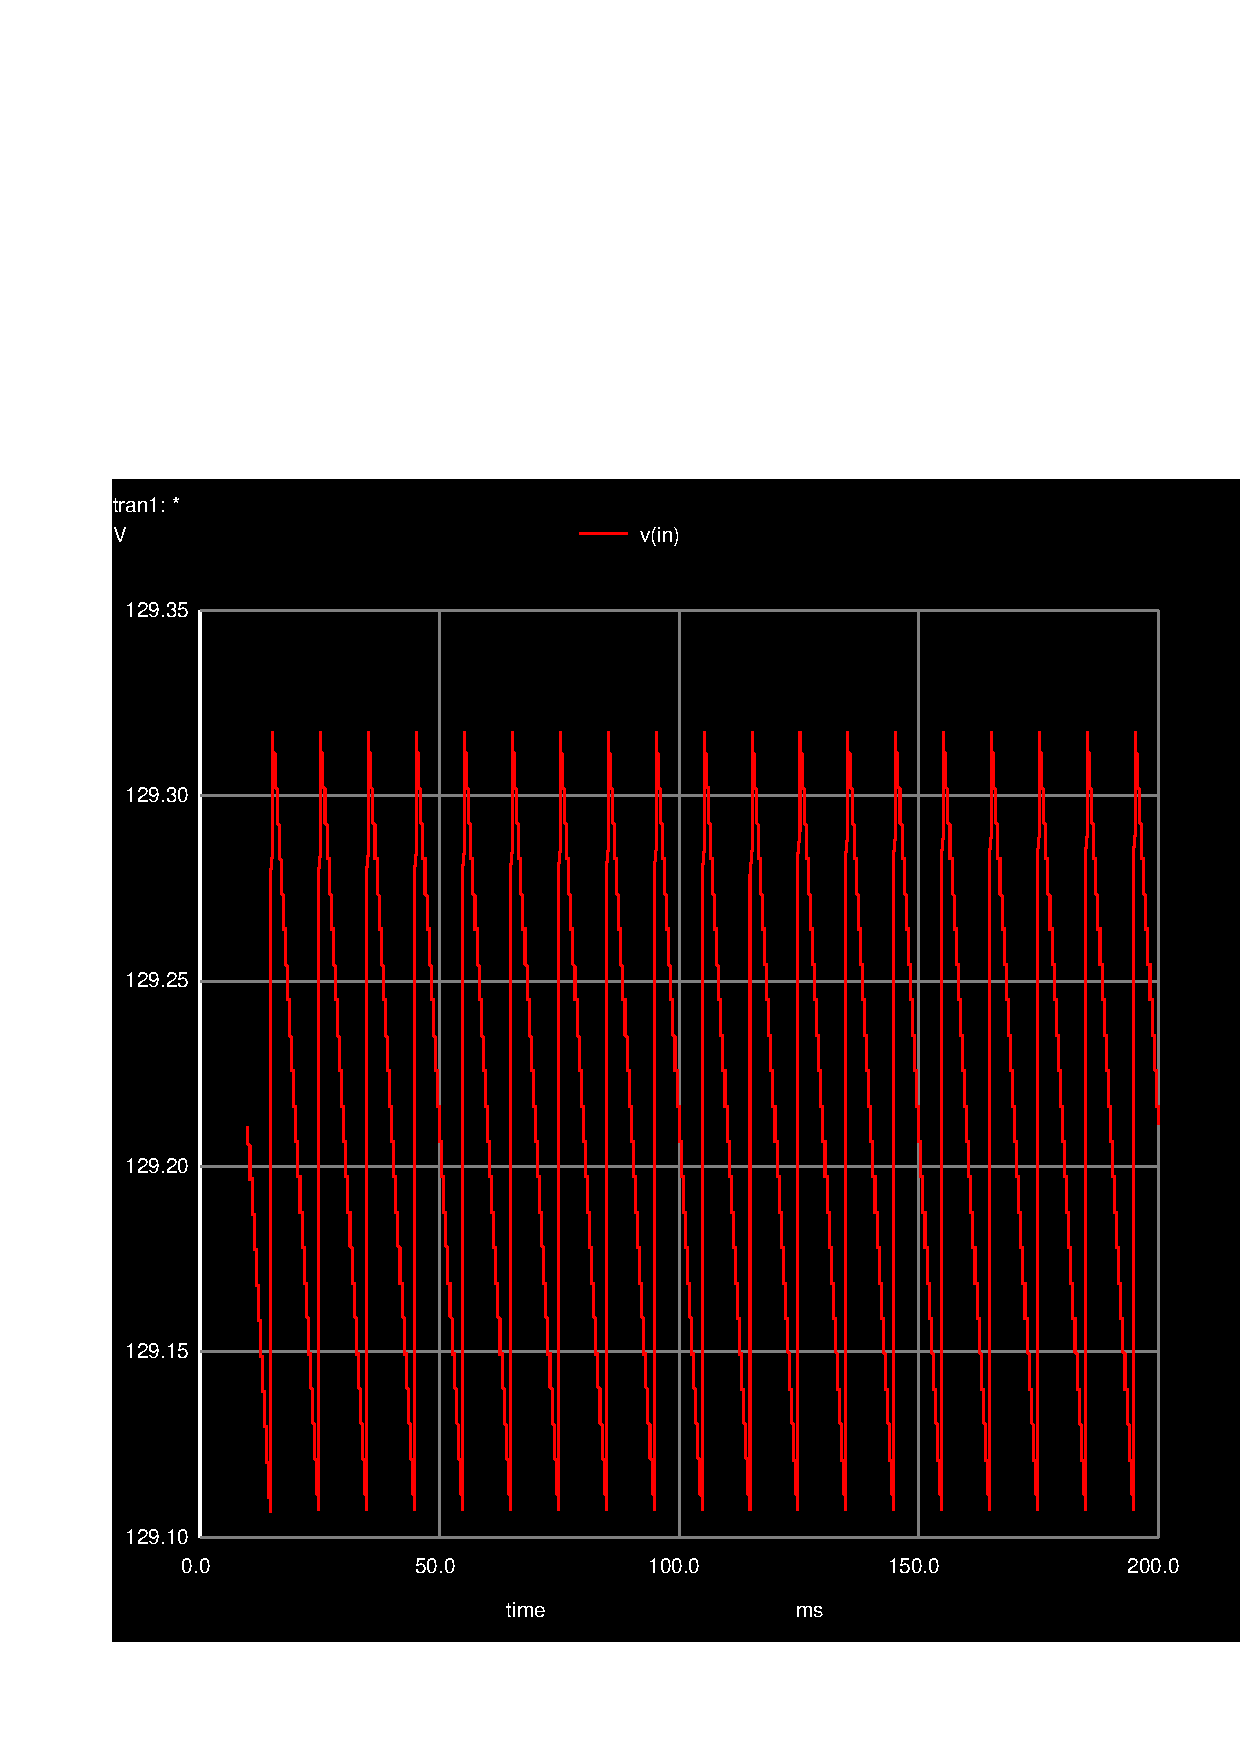
\includegraphics[height=12cm]{../sim/trans41.pdf}
	\caption{$v_{IN}(t)$ ($v_{Envelope}(t)$)}
	\vspace{-3cm}
\end{figure}

\newpage

\begin{figure}[h] \centering
	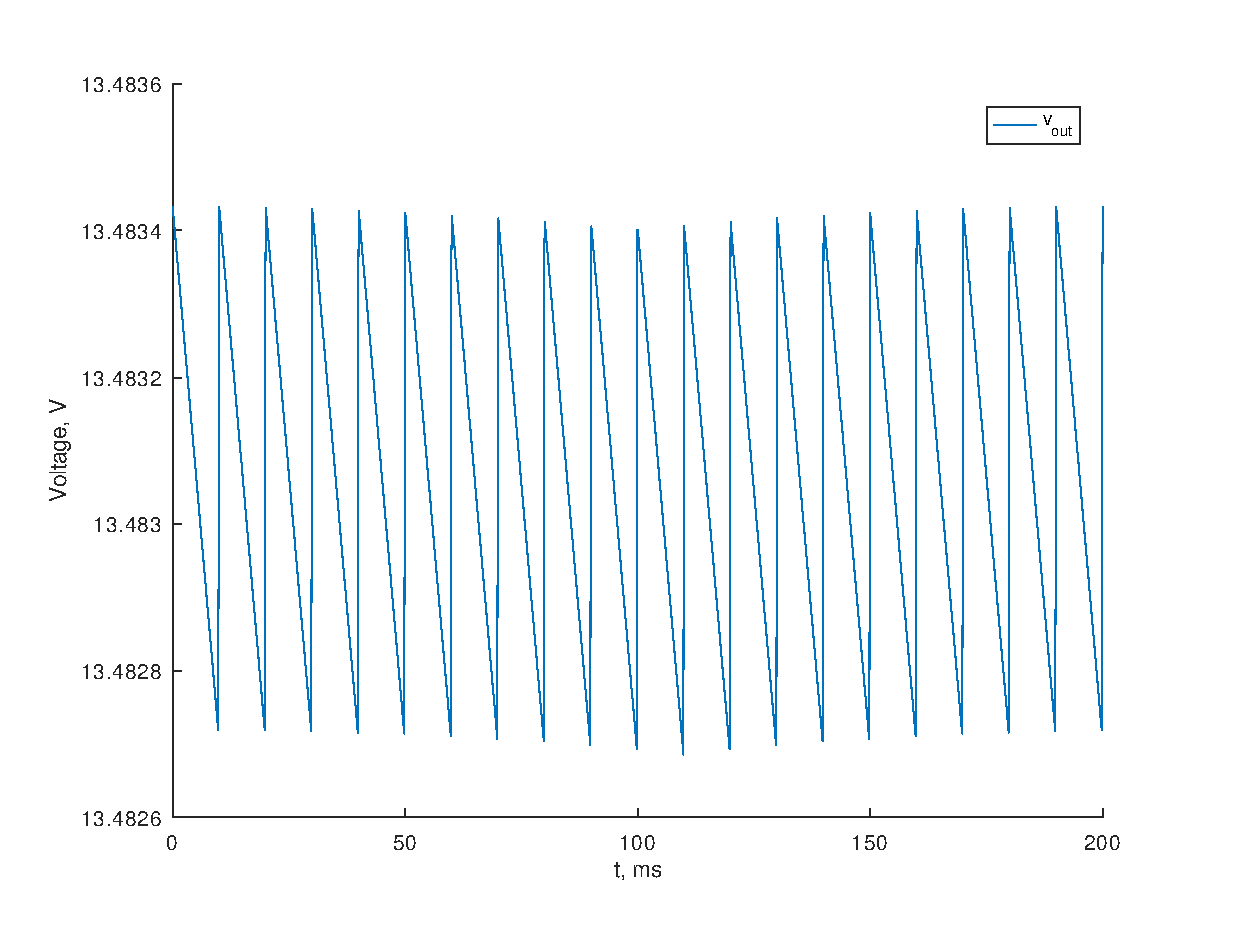
\includegraphics[height=8cm]{PASSO42.eps}
	\caption{$V_{out}$.}
\end{figure}
  	
\begin{figure}[h] \centering
	\vspace{-2cm}
	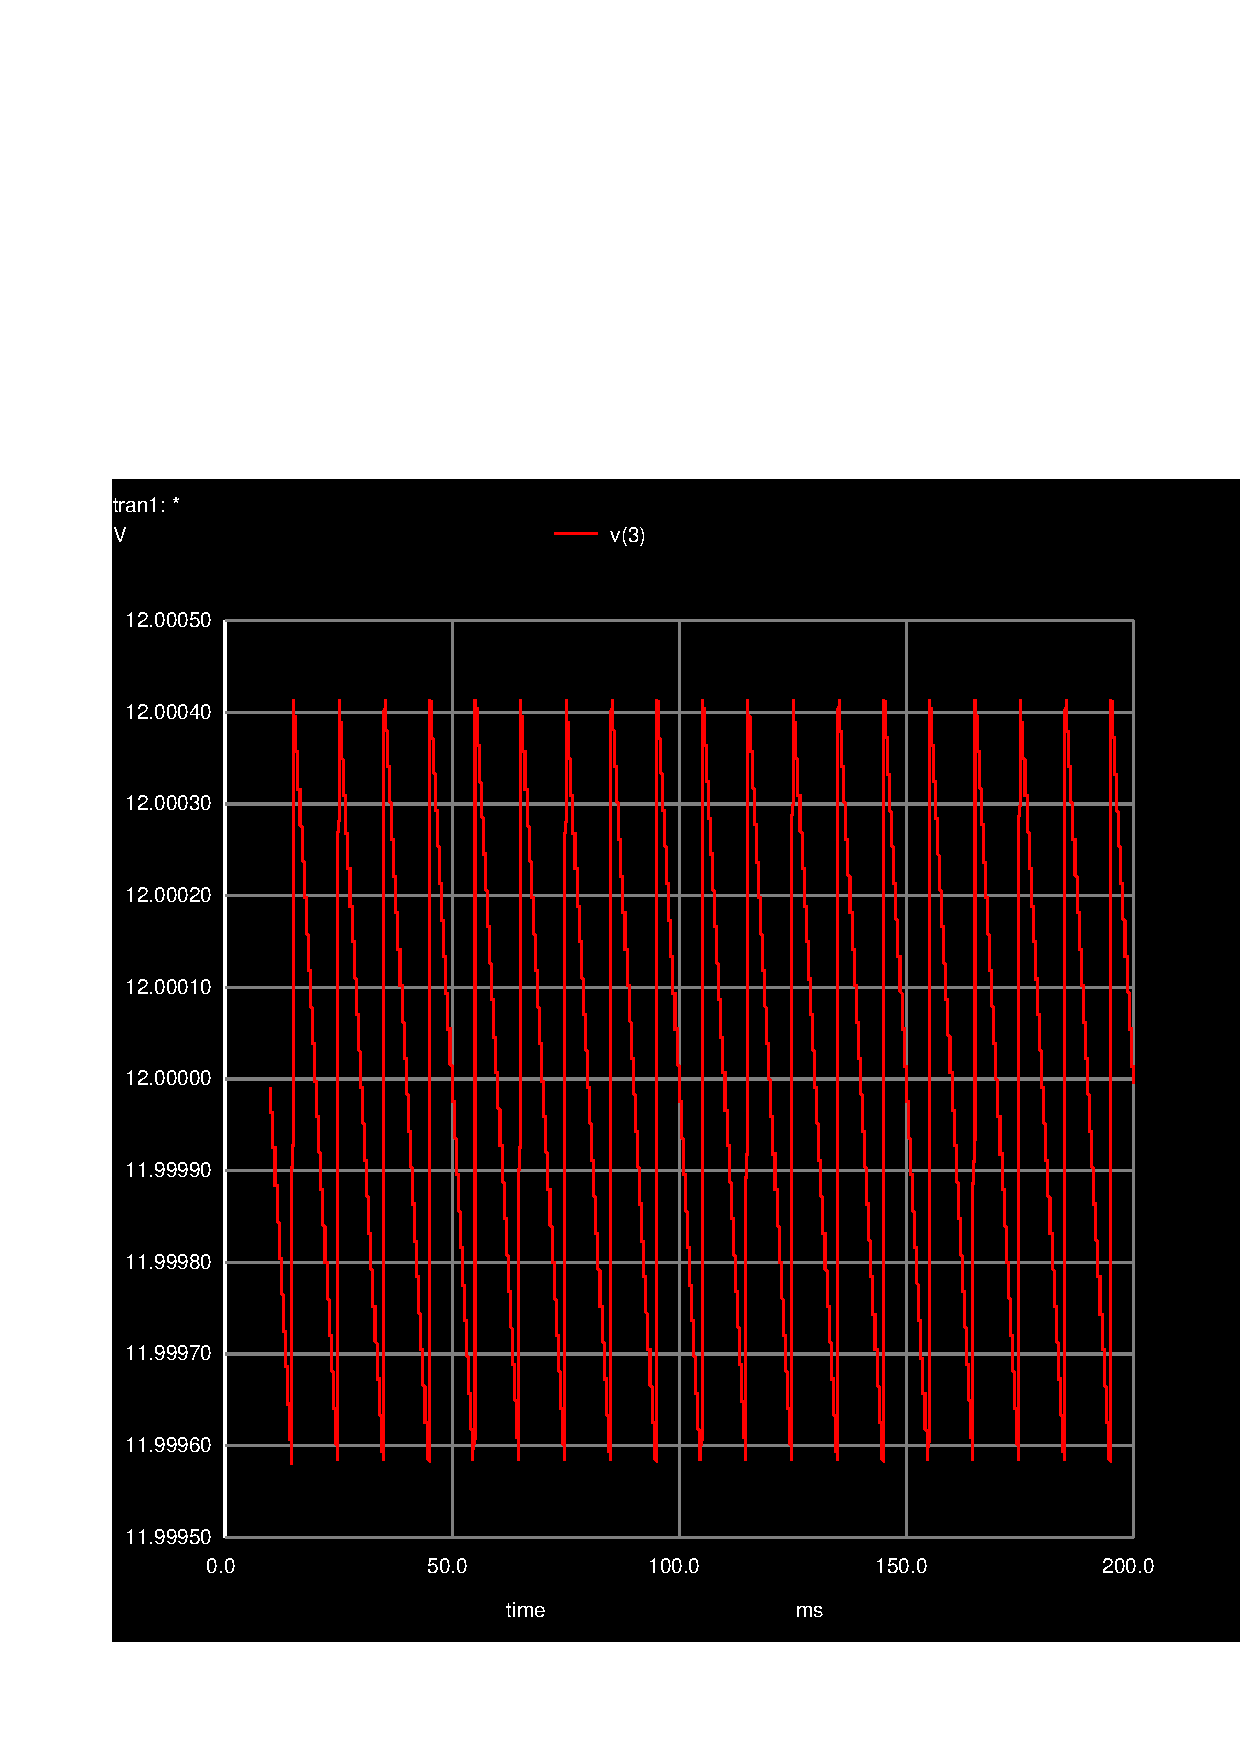
\includegraphics[height=12cm]{../sim/trans42.pdf}
	\caption{$v_{3}(t)$ ($v_{OUT}(t)$)}
	\vspace{-3cm}
\end{figure}

\newpage

\begin{figure}[h] \centering
	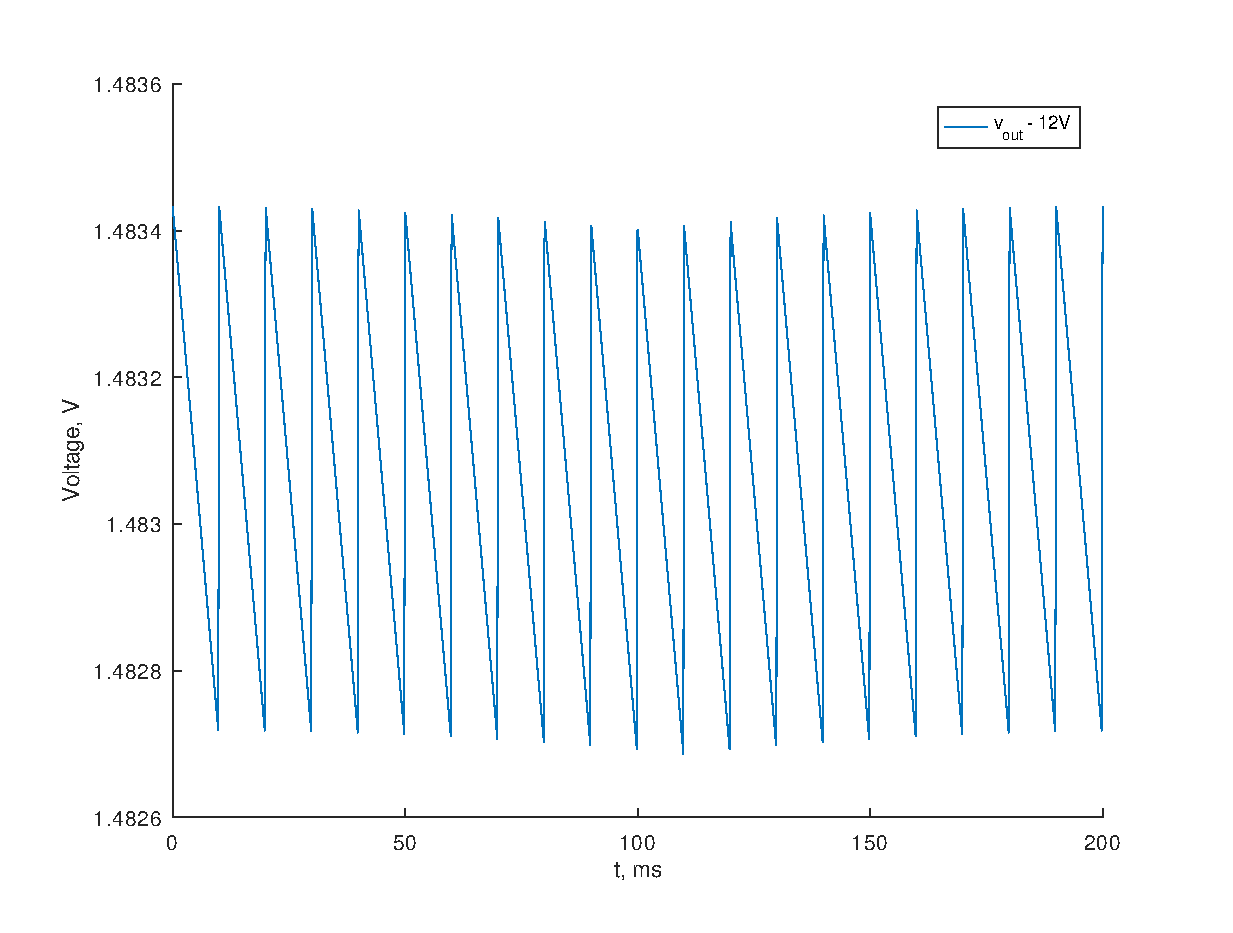
\includegraphics[height=8cm]{PASSO5.eps}
	\caption{$V_{out} - 12V$.}
\end{figure}
  	
\begin{figure}[h] \centering
	\vspace{-2cm}
	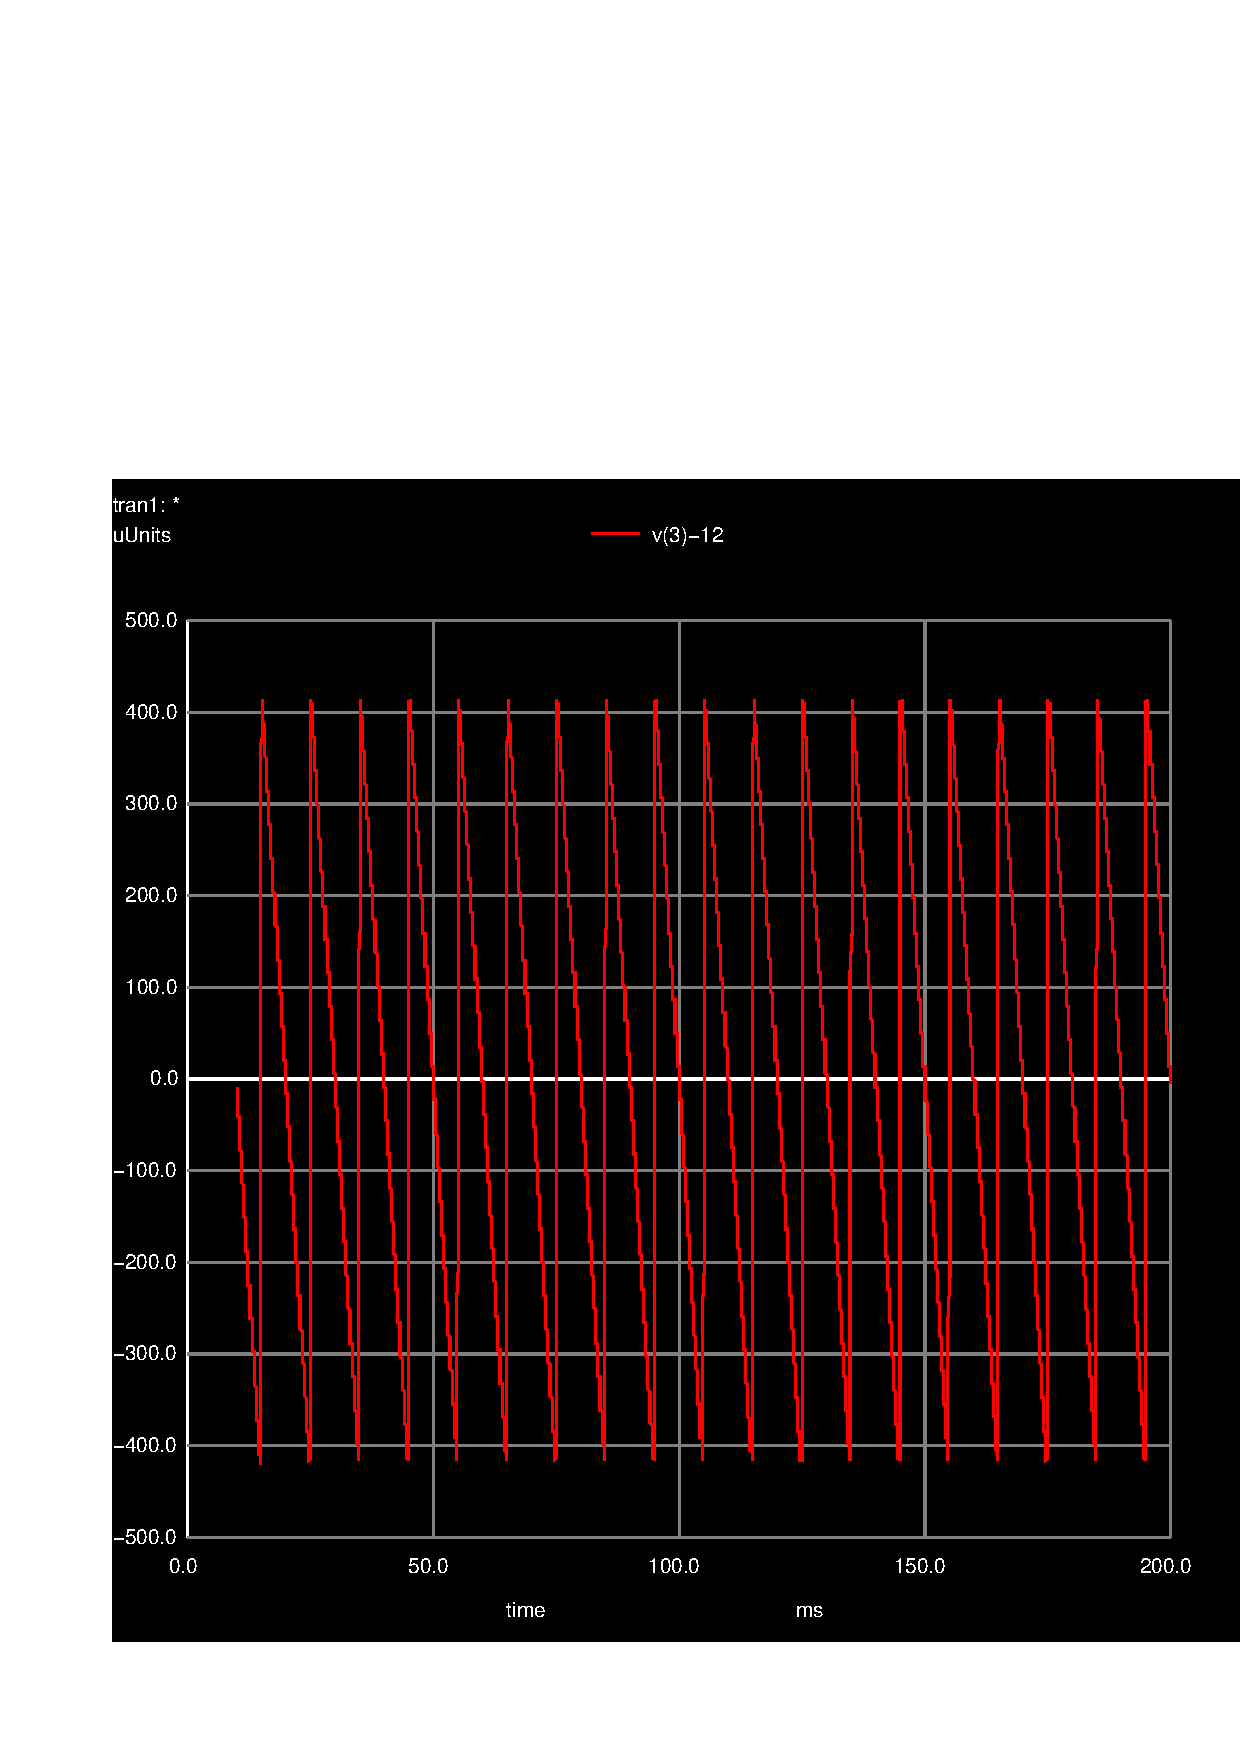
\includegraphics[height=12cm]{../sim/trans5.pdf}
	\caption{$v_{3}(t)-12$ ($v_{out}(t)-12$)}
	\vspace{-3cm}
\end{figure}

\newpage

\begin{figure}[h] \centering
	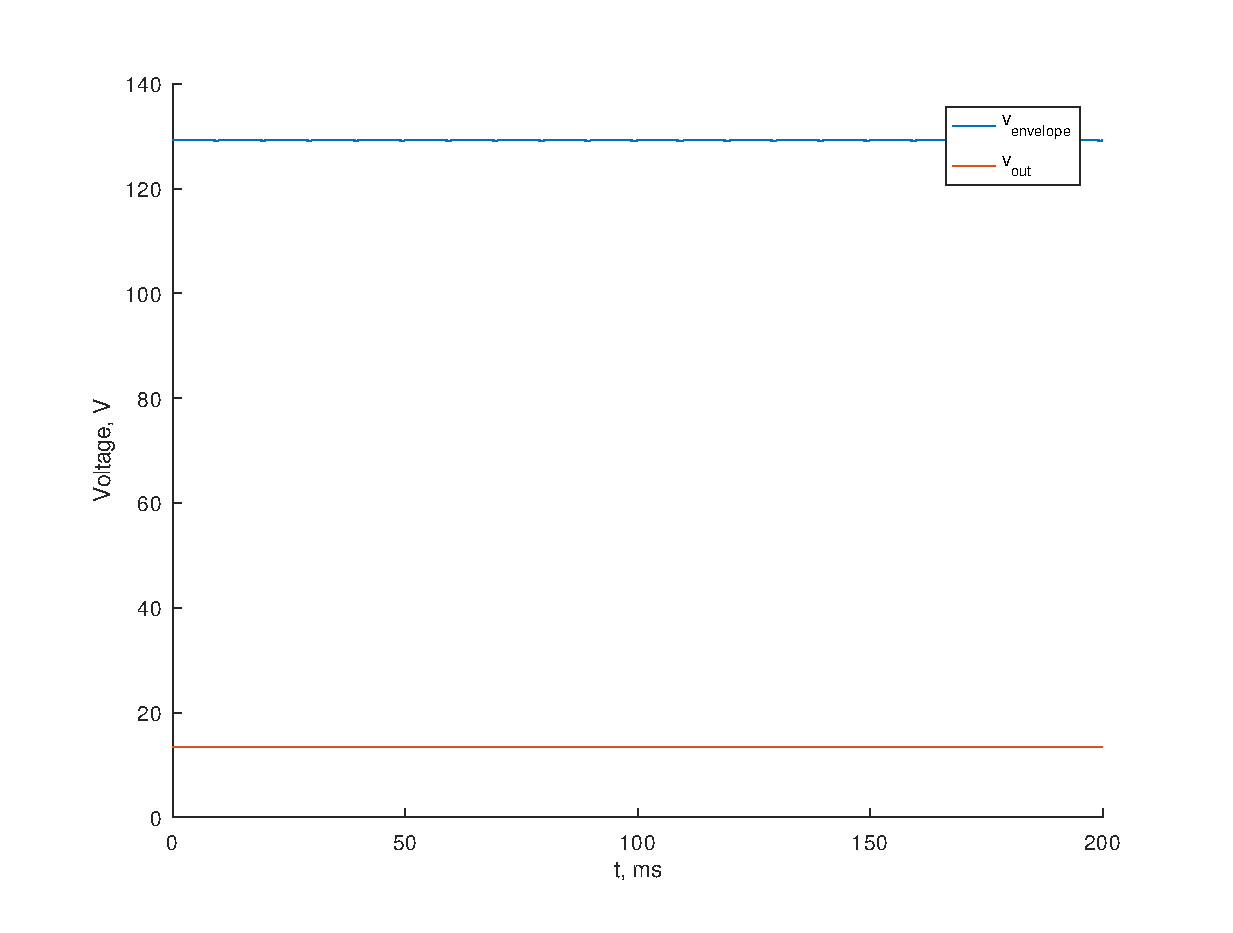
\includegraphics[height=8cm]{PASSO4.eps}
	\caption{$V_c$ and $V_{out}$.}
\end{figure}
  	
\begin{figure}[h] \centering
	\vspace{-2cm}
	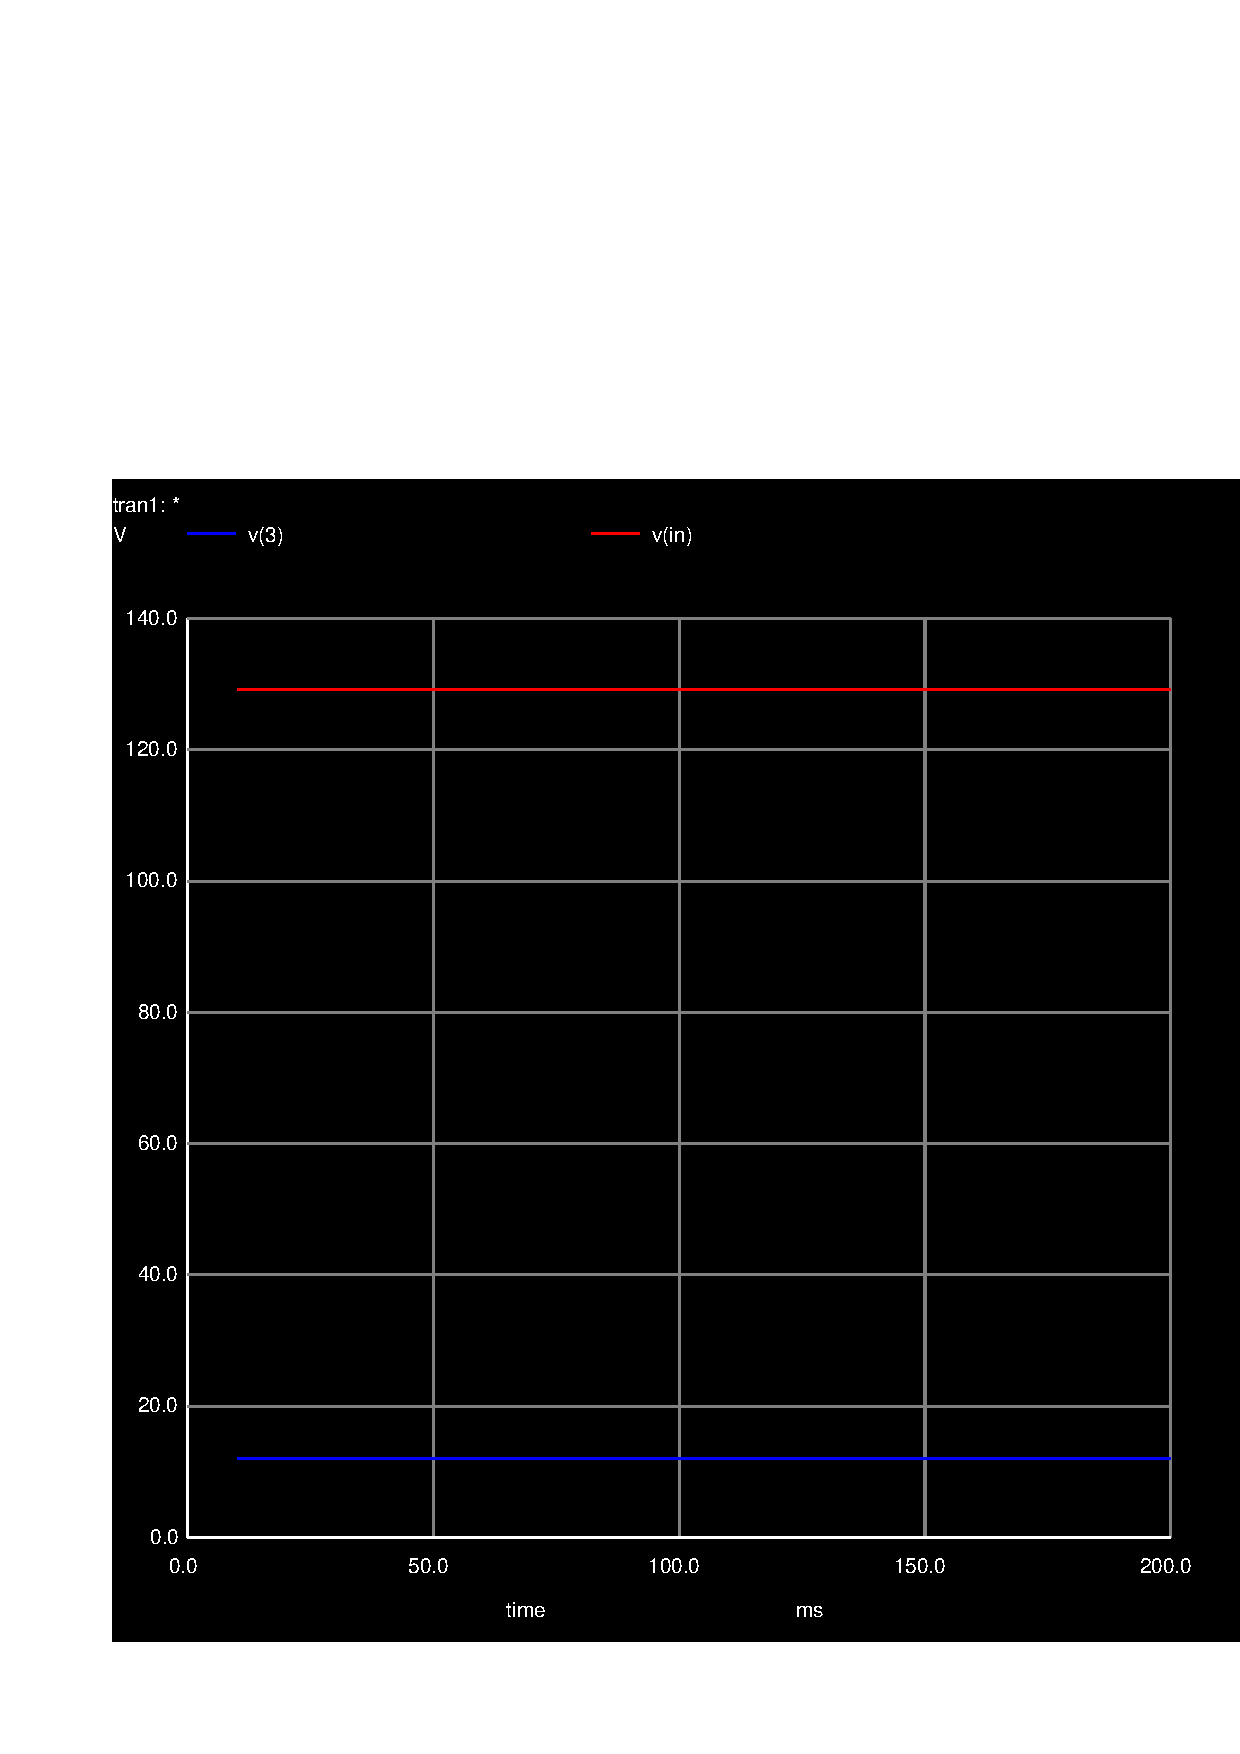
\includegraphics[height=12cm]{../sim/trans4.pdf}
	\caption{$v_3(t)$ ($v_{OUT}(t)$) and $v_{IN}$ ($v_{Envelope}(t)$)}
	\vspace{-3cm}
\end{figure}
